\DeclarePairedDelimiter\norm{\lVert}{\rVert}

\section{Creature Generation}
\subsection{Parametrische Kreatur}
Als Grundlage für die parametrische Generierung der Kreaturen dient das von Jon Hudson in seiner Thesis \cite{Hudson2013CreatureGU} beschriebene Modell, welches in Abschnitt \ref{} näher beschrieben wird.\\
Die Kreatur besteht aus mehreren Körperteilen, die separat generiert werden und jeweils ihre eigenen Parameter besitzen. Diese Körperteile sind Torso, Beine, Arme, Hals, Füße und Kopf, die jeweils aus einem oder mehreren Knochen bestehen. Alle in diesem Abschnitt erwähnten Zufallsvariablen entstammen einer uniformen Verteilung.

\subsubsection{Knochen Koordinaten}
Um einfache lokale Transformationen zu ermöglichen, definieren wir ein einheitliches Koordinatensystem für alle Knochen. Der Ursprung dessen ist der \textbf{proximale Punkt}, dieser ist der der Körpermitte am nächsten gelegene Punkt und entspricht somit der Stelle, an der der knochen, gegebenenfalls mit einem Offset, an seinem Elternknochen befestigt ist. Der \textbf{distale Punkt} ist der Endpunkt des Knochens, also der am weitesten von der Körpermitte entfernte Punkt. \\ Die \textbf{proximale Achse} verläuft parallel zum Knochen, von der Körpermitte weg, also in Richtung des distalen Punktes. Die \textbf{ventrale Achse} liegt orthogonal zur proximalen Achse und zeigt in Richtung der Vorderseite des Knochens. Diese lässt sich prinzipiell beliebig definieren, in unserem Fall haben wir uns jedoch für Armknochen auf die dem Körper zugewandte Innenseite des Knochens festgelegt, für parallel zum Boden generierte Torsi auf die Unterseite und für alle weiteren Knochen auf die der Blickrichtung des Skeletts zugewandten Seite. Die \textbf{laterale Achse} liegt senkrecht auf den beiden zuvor definierten Achsen.

\subsubsection{Generierung}
Unsere Methode setzt voraus, dass zunächst gewisse Vorgaben zur generellen Struktur der Kreatur gemacht werden. In unserem konkreten Fall bedeutet dies, dass wir uns zunächst auf Zwei- und Vierbeiner beschränken. Der Zweibeiner orientiert sich an der menschlichen Anatomie und besitzt deshalb in jedem Bein jeweils zwei Knochen und einen einzelnen Fußknochen sowie zwei Arme. Die Beine eines Vierbeiners besitzen, angelehnt an die Skelette echter vierbeiniger Säugetiere, jeweils vier Knochen. Arme werden hier nicht generiert. Um Kreaturen zu erzeugen, die nicht einer dieser Strukturen entsprechen, wie beispielsweise Spinnentiere oder Echsen, müsste man weitere Skelette definieren.\\
\\
Zuerst  wird der \textbf{Torso} Generiert. Im Falle des Zweibeiners ist dieser nach oben gerichten, beim Vierbeiner parallel zum Boden. Als Parameter werden jeweils Minima und Maxima für die Länge und den Umfang des Torsos übergeben. Daraus wird zunächst ein zufälliger Wert für die Länge bestimmt. Da wir uns vorerst für einen Torso bestehend aus drei Knochen entschieden haben, wird diese Länge zufällig auf drei kleinere Längen aufgeteilt. Jeder dieser Knochen erhält dann einen zufälligen Umfang. Das unterste Torsosegment dient als Elternknochen der Kreatur, die anderen beiden Knochen werden dann nacheinander am distalen Punkt des vorangegangenen Knochens befestigt.\\
Anschließend werden die \textbf{Beine} paarweise generiert, wodurch nur symmetrische Kreaturen erstellt werden können. Auch hier wird zunächst die Länge zufällig bestimmt und dann auf zwei beziehungsweise vier Knochen aufgetelt. Auch Die Umfänge werden zufällig bestimmt, jedoch zusätzlich sortiert, sodass das das dickste Segment der Körpermitte am nächsten gelegen ist. In beiden Fällen werden die Beine gerade nach unten gereriert. Bei einem Zweibeiner wird am distalen Punkt des unteren Beinknochen in Richtung dessen ventraler Achse ein Fußknochen mit parametrisch zufällig bestimmter Größe erzeugt. Befestigt werden die Beine durch einen zusätzlichen Hüftknochen, der parallel zum Torso am proximalen Punkt des ersten Torsoknochens ansetzt und dessen proximale Achse entgegen derer seines Elternknochens gerichtet ist, also den Torso etwas verlängert. Es wird jeweils ein Bein links und rechts vom Mittelpunkt des Hüftknochens angebracht. Der Abstand entlang der lateralen Achse ergibt sich aus dem Umfang des Knochens. Im Falle des Vierbeiners wird analog dazu ein weiteres Beinpaar am distalen Punkt des letzten Torsoknochens generiert. Anschließend werden Torso und Beine so rotiert, dass sich alle Enden der Beine auf der selben Höhe befinden und die Beine noch immer gerade nach unten Zeigen.\\
Die \textbf{Arme} des Zweibeiners werden analog zu den Beinen mit Hilfe eines Schultersegmentes am distalen Punkt des obersten Torsoknochens erzeugt.\\
Der \textbf{Hals} wird als Verlängerung des Torsos generiert. Dabei wird sowohl die Länge und Dicke zufällig bestimmt als auch die Anzahl der Knochen. Beim Zweibeiner wird er am distalen Punkt des Schulterknochens befestigt und alle Knochen zeigen parallel zum Torso gerade nach oben. Beim Vierbeiner erfolgt das Befestigen am distalen Punkt des vorderen Hüftknochens. Dabei ist die Rotation des ersten Knochens ein zufälliger Wert zwischen der der proximalen und der der negativen ventralen Achse des Elternknochens. Jedes weitere Halssegment erhält eine zufällige Rotation um $\pm 20\degree$.\\
Der \textbf{Kopf} ist ein einzelner Knochen mit zufälliger Länge und Umfang, der als Verlängerung des letzten Halsknochens betrachtet werden kann.\\
\\
Die glaubwürdigkeit und Variation der Kreaturen ist dadurch also auch stark von den gewählten Parametern Abhängig. Diese werden von Hand gesetzt, wobei größere Wertebereiche auch für größere Unterschiede zwischen den Kreaturen sorgen, aber gleichzeitig die Kontrolle über das Ergebnis einschränken. Die Beschränkungen der Bewegungsradii der Gelenke werden momentan händisch mit erfahrungsgemäß guten Werten gesetzt. Ziel ist es allerdings auch diese in Zukunft soweit möglich prozedural mit Hilfe von Parametern zu erzeugen, um verschiedene Bewegungsmuster zu ermöglichen.




\subsection{L-System Creature}
% Vom L-System zu den Knochen (Strecken) -> Rotation um die Achsen mittels Euler->Quarternion
\subsubsection{Generierung der Skelettstruktur}

%Nach Subsubsection "Generierung der Skelettstruktur"
\subsubsection*{Skelett aus L-System generieren}
Ausgehend von einer Liste von Tupeln, die jeweils Start und Endpunkte einer von der Turtle gezeichneten Strecke enthalten wird das Skelett mit Unity Klassen generiert. Zunächst wird die Liste in eine Baumstruktur überführt. Dabei entspricht ein Knoten im Baum einem Knochen im Skelett. Zwei Knoten stehen in einer Eltern-Kind-Beziehung im Baum, wenn die zugehörigen Strecken sich schneiden. Dabei wird gefordert, dass der Endpunkt der zum Elternknoten gehörigen Strecke dem Startpunkt der zum Kindknoten gehörigen Strecke gleicht. Da angenommen wird, dass es zu jedem Startpunkt eines Tupels in der Liste ein weiteres Tupel gibt, dessen Endpunkt dem Startpunkt gleicht lässt sich der Baum so definieren. Der Baum wird traversiert und zu jedem Knoten wird ein GameObject erstellt.  Dieses wird mit einem Rigidbody, einem CapsuleCollider und einem primitiven Mesh versehen. Die Knochen werden in Kategorien, wie zum Beispiel Arm, Bein oder Kopf eingeteilt. Zwei Knochen werden mit einem Joint verbunden, wenn sie im Baum in einer Eltern-Kind-Beziehung stehen. Für die erlaubten Rotationen der Joints wurden Standardwerte je nach Kategorie festgelegt. Abbildung \ref{skeletonlsystemex} zeigt ein über ein L-System generiertes Skelett.

\begin{figure}[h]
\begin{center}
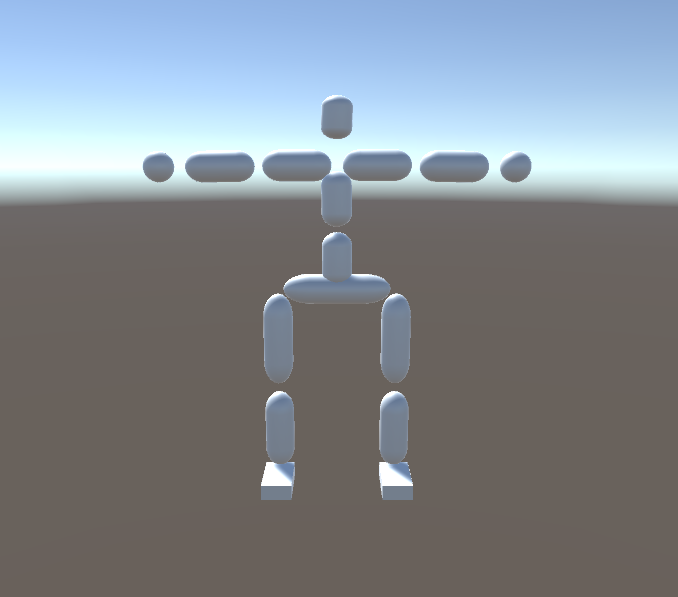
\includegraphics[width = 0.5\textwidth]{resources/img/skeletonlsystemex.png}
\end{center}
\caption{Mittels L-System generiertes Skelett}
\label{skeletonlsystemex}
\end{figure}


\subsection{Mesh-Generierung}
\subsubsection{Metaball}
Zur Generierung der Geometrie der Kreatur verwenden wir, angelehnt an den Ansatz von Madis Janno \cite{Janno20182dCG} (siehe Abschnitt \ref{sec:metaball}), eine modifizierte Form von Metaballs. Dabei werden genau so viele Bälle entlang eines Generierten Segments platziert wie benötigt werden um zu garantierten, dass dadurch in jedem Fall ein zusammenhängendes Mesh entsteht. Tatsächlich ist jedoch der Einfluss nahegelegener Kugeln aufeinander so groß, dass dadurch nicht nur die minimale Berührung der einzelnen Kugeln entsteht, sondern diese glatt ineinander übergehen. Wie auch bei Janno lässt sich unsere Methode mit beliebigen Metaball-Funktionen durchführen. Aufgrund der guten Ergebnisse haben wir uns jedoch vorerst auf die gleiche, zuerst von Ken Perlin beschriebene, Falloff-Funktion festgelegt.
\[f_i(\vec{x}) = exp(B_i - \frac{B_ir_i^2(\vec(x))}{R_i^2})\]
Für Metaball $i$ ist $R_i$ dessen Radius, $B_i$ ein Parameter zur Einstellung der "Blobbiness", welcher beeinflusst wie sehr sich Metaballs miteinander verbinden. Wir verwenden den Wert $B_i = 0.5$. $r_i(vec{x})$ ist der Abstand des Punktes $\vec{x}$ zum Zentrum $c_i$ von Metaball $i$, also: \[r_i(\vec{x})=||\vec{x}-\vec{c_i}||=\sqrt{(x_x-c_{ix})^2+(x_y-c_{iy})^2+(x_z-c_{iz})^2}\]

Die generierten Kreaturen bestehen aus mehreren Segmenten (Knochen) mit jeweils einem Start- und Endpunkt sowie einer Dicke, die als Radius der darauf platzierten Metaballs verwendet werden kann. Entlang dieser Segmente soll dann das Mesh erzeugt werden. Die von Janno beschriebene Methode berechnet dafür, abhängig von der gewählten Falloff-Funktion, die minimale Anzahl an Metabällen für ein Segment und platziert diese gleichmäßig entlang dessen. Das Problem, welches sich daraus bei unseren Experimenten ergeben hat, liegt darin, dass mit höherer Komplexität der Kreaturen und einer damit einhergehenden steigenden Anzahl an Segmenten, der Einfluss von benachbarten Segmenten nicht gut kontrollieren lässt und diese teilweise ineinander verschmelzen. \\

Unser Ansatz um dieses Problem zu umgehen ist es, die Anzahl der einzelnen Metabälle drastisch zu reduzieren. Anstatt einer beliebig großen Zahl an Bällen entlang jedes Segments, erzeugen wir jeweils nur einen einzigen Körper. Dazu ersetzen wir die Bälle durch Kapseln, also Zylinder mit jeweils durch eine Halbkugel abgerundeten Enden, weshalb wir diese auch als "Metakaspeln" bezeichnen. Möglich macht uns dies eine Modifikation der Falloff-Funktion, beziehungsweise der darin verwendeten Distanz. Wir berechnen hierbei nicht den Abstand zum Zentrum einer Kugel, sondern zu der Verbindungslinie zwischen Start- und Endpunkt. \\

\begin{figure}[ht]
\centering
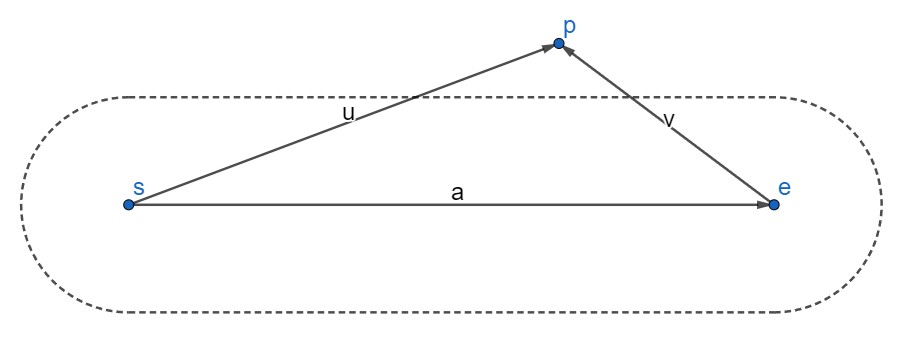
\includegraphics[width=0.7\textwidth]{resources/img/metacapsule.png}
\caption{Beispiel Metakapsel; Die gestrichelte Linie enthält alle Punkte mit $r=R$}
\label{metacapsule}
\end{figure}

Um diese Form zu erzeugen muss lediglich die Funktion $r(\vec{x})$ zur Berechnung des Abstandes angepasst werden.
Sei $s$ der Startpunkt, $e$ der Endpunkt, $a$ der Vektor $e-s$, $p$ ein Punkt, dessen Abstand berechnet werden soll, $u=p-s$ und $v=p-e$ (Siehe Abbildung \ref{metacapsule}). Die Distanz lässt sich dann folgendermaßen bestimmen:
\[
    r(\vec{x})= 
\begin{cases}
    ||p-s||,& \text{falls } a\cdot u < 0\\
    ||p-e||,& \text{falls } a\cdot v > 0\\
    \norm*{\frac{a\times u}{\norm{a}}},& \text{sonst}
\end{cases}
\]

Es werden drei Fälle unterschieden. Liegt der Punkt $p$ im Falle von Abbildung \ref{metacapsule} links von $s$, beziehungsweise rechts von $e$, ist Die Distanz von $p$ zum Segment einfach der euklidische Abstand zum jeweiligen Punkt. Ob dies der Fall ist, lässt sich mit Hilfe der Skalarprodukte $a\cdot u$ beziehungsweise $a\cdot v$ überprüfen. Ansonsten berechnet man die Distanz von Punkt p zur Geraden, die durch $s$ und $e$ verläuft.\\

Da dies nur eine Erweiterung der Metaball-Funktion ist, lassen sich diese Kapseln weiterhin mit anderen Metabällen kombinieren. So können auch Körperteile erstellt werden, die nicht aus solchen Segmenten bestehen, oder Details aus kleineren Metabällen entland der Segmente platziert werden. Grundsätzlich lassen sich auf diese Weise beliebig geformte Objekte, die mit einer solchen Funktion definiert werden, einbinden.
Da die Kapsel nur zylindrisch geformte Segmente darstellen lässt, die in alle Richtungen den gleichen Radius besitzen, haben wir eine weitere Modifikation vorgenommen, die es erlaubt die Metakapsel entlang der ventralen oder lateralen Achse zu strecken beziehungsweise zu stauchen. Dadurch ist es uns möglich Körperteile mit unterschiedlichen Abmessungen entlang der verschiedenen Achsen darzustellen und dennoch unnatürlich wirkende Formen wie beispielsweise einen Quader zu vermeiden.
Dazu bestimmen wir bei der Berechnung von $r(\vec{x})$ zunächst den Vektor, der die kürzeste Verbindung von $\vec{x}$ und dem Segment darstellt, anstatt direkt dessen Länge auszuwerten. Diesen Vektor skalieren wir anschließend entlang der gewünschten Achse. Die Länge des skalierten Vektors ist dann die neue Distanz.


\subsubsection{Marching Cubes}
TODO: wollen wir hier noch etwas genauer drauf eingehen, oder reicht der Teil von Jona???

\subsubsection{Mesh Indexing}
Zur weitere Verarbeitung des Meshes beim automatischen Rigging, ist es wichtig, dass das Mesh korrekt indiziert ist, sodass keine doppelten Vertices existieren. Außerdem können so die ausgehenden Kanten der Vertices bestimmt werden, welche ebenfalls später für das automatische Rigging benötigt werden. Während dem Marching Cubes Algorithmus werden die entstehende Dreiecke in eine gesonderte Datenstruktur hinzugefügt, welche für jeden Vertex prüft, ob dieser bereits im Vertex-Buffer existiert. Falls ja, wird kein neuer Vertex eingefügt, sondern das Dreieck referenziert den Vertex über den Index-Buffer. Neue Vertices werden dem Vertex-Buffer hinzugefügt und das entsprechende Dreieck referenziert den neuen Vertex. Die Anzahl der Vertices wird dadurch außerdem signifikant verringert, was Performance-Vorteile beim Rendering und bei der Weiterverarbeitung des Meshes ermöglicht.

\subsubsection{Delaunay Triangulation}
In der Entwicklung des automatischen Riggings des Modells wurde festgestellt, dass die Triangulierung des Meshes, welches durch Marching Cubes entsteht nicht numerisch stabil genug ist, um mit der Bone-Heat Methode die Vertex-Gewichte zu berechnen. Für die Lösung des Matrix-Systems der Bone-Heat Methode ist es wichtig, dass die Triangulierung die Delaunay-Bedingung erfüllt~\cite{laplace_beltrami_paper}.

Eine Delaunay-Triangulierung maximiert das Minimum von allen Winkeln in der Triangulierung~\cite{delaunay}. Diese Triangulierung vermeidet Dreiecke die extrem lang und dünn sind. Eine Triangulierung erfüllt die Delaunay-Bedingung genau dann wenn der Umkreis jedes Dreiecks leer ist.

Die Triangulierung, die bereits durch den Marching Cubes Algorithmus entstanden ist, kann durch die `Edge-Flipping' Technik in eine Delaunay Triangulierung transformiert werden~\cite{delaunay}. Dazu iteriert der Algorithmus durch alle Kanten des Meshes und prüft für die beiden anliegenden Dreiecke der Kante, ob die gegenüberliegenden Winkel $\alpha$ und $\beta$ kleiner oder gleich $180\degree$ sind. Die Bedingung $\alpha+\beta \leq 180\degree$ ist equivalent zu der Delaunay-Bedingung der beiden Dreicke. Wenn die Delaunay-Bedingung nicht erfüllt ist, können die Dreiecke durch eine `flip' Operation korrigiert werden. Dabei die gemeinsame Kante $BD$ der Dreiecke $\triangle ABD$ and $\triangle BCD$ in eine Kante $AC$ mit Dreiecken $\triangle ABC$ and $\triangle ACD$ geändert. Für das gesamte Mesh kann einfach so lange die `flip' Operation ausgeführt werden, bis alle Dreiecke delaunay sind.

Die `edge-flip' Operation ist auf der Mesh-Datenstruktur, welche in 3D-Engines wie Unity verwendet wird relativ aufwendig, da diese keine Möglichkeit bietet, um die Dreiecke einer Kante zu finden. In diesem Projekt wurde daher die Polygon Mesh Processing Bibliothek (PMP)~\cite{pmp-library} verwendet. Diese enthält bereits viele Methoden um 3D-Meshes auf komplexe Weise zu modifizieren. Insbesondere wird eine optimierte Datenstruktur für das Mesh genutzt, welche es erlaubt schnell über alle Kanten zu iterieren und diese ohne großen Aufwand zu flippen.

\subsection{Automatisches Rigging}
Um die Bone-Struktur des generierten Skelettes mit dem Mesh zu verknüpfen, muss bei der 3D-Modellierung der Prozess des Riggings durchlaufen werden. Dieser beschreibt wie sich jeder einzelne Vertex des Meshes mit den Bones in der Szene bewegt. Jeder Vertex kann an beliebig vielen Bones angehängt werden. Durch eine Gewichtung wird bestimmt wie sehr ein Vertex durch der Transformation eines Bones mitbewegt wird.
Da sowohl das Skelett, als auch das gesamte Mesh prozedural generiert werden, kann das Rigging nicht wie üblich in einem Modellierungs-Tool wie Blender~\cite{blender} manuell durchgeführt werden, sondern muss zur Laufzeit des Spiels während der Generierung der Kreaturen geschehen.

Für ein erfolgreiches Rigging ist es wichtig, dass das Skelett bereits sinnvoll in dem Mesh eingebettet ist. Da hier das Mesh aus Metaballs generiert wird, welche um die Bones plaziert sind, können wir hier davon ausgehen, dass das Mesh das Skelett bereits \emph{sinnvoll} umhüllt.

\begin{figure}[h!]
	\centering
	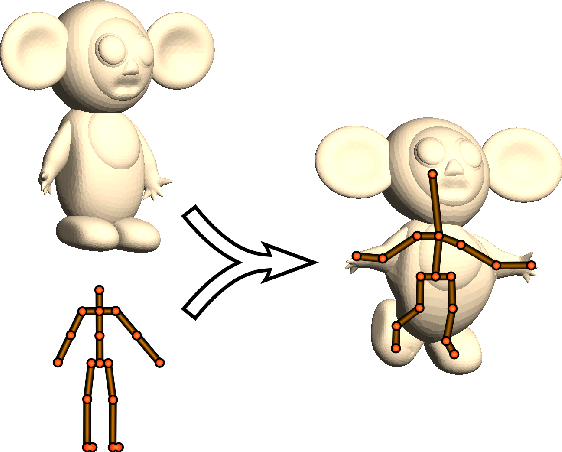
\includegraphics[width=0.6\linewidth]{resources/img/skeleton_embedding.png}
	\caption{Beispiel für ein korrekt eingebettetes Skelett in einem Mesh~\cite{bone_heat_paper}.}
	\label{fig:skeleton_embedding}
\end{figure}

Während der Entwickelung wurde zunächst eine triviale Methode als Zwischenlösung verwendet. Dabei wurden alle Vertices nur an den Bone mit der geringsten Distanz angehängt. Diese Methode ist jedoch visuell nicht brauchbar, da bei Bewegung des Skeletts an den Gelenken zwischen den Bones Löcher und verschiedene andere Artefakte entstehen. Es wird also eine Lösung benötigt, die es ermöglicht Vertices an mehrere Bones anzuhängen und die Gewichte so bestimmt, dass das Mesh an den Übergängen zwischen den Bones möglichst natürlich deformiert wird.

\subsubsection{Bone-Heat Methode}
Ein bereits bekannter Algorithmus zur automatisch Gewichtsberechnung und Verknüpfung des Meshes ist die Bone-Heat Methode~\cite{bone_heat_paper}. Dieser berücksichtig mehrere zusätzliche Eigenschaften für die Gewichte. Zuerst sollen die Gewichte unabhängig von der Auflösung des Meshes sein. Außerdem müssen die Gewichte sich sanft über den Verlauf der Oberfläche verändern. Die Breite des Übergangs zwischen zwei Bones sollte ungefähr proportional zu der Distanz des Gelenks zur Oberfläche des Meshes sein.
Ein Algorithmus, welcher die Gewichte alleine aus der Distanz der Bones zu den Vertices berechnet, kann oft schlechte Ergebnisse liefern, da er die Geometrie des Modells ignoriert. Zum Beispiel können Teile des Torsos mit einem Arm verbunden werden. Die Bone-Heat Methode behandelt stattdessen das innere Volumen des Modells als einen wärmeleitenden Körper. Es werden für jeden Vertex die Gleichgewichts-Temperatur berechnet und diese als Gewichte für die Bones verwendet. Wie in Abbildung~\ref{fig:bone_heat_equilibrium} zu sehen ist, wird ein Bone auf 1° gesetzt und der andere auf 0°. Bei Deformation der beiden Bones mit den Gewichten aus dem Temperatur-Gleichgewichts entsteht an dem Gelenk eine natürlich aussehende Verformung der Oberfläche.

\begin{figure}[h!]
	\centering
	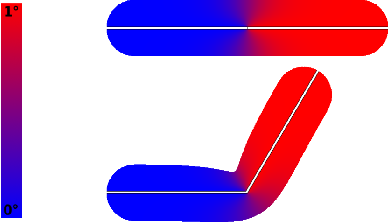
\includegraphics[width=0.7\linewidth]{resources/img/bone_heat_equilibrium.png}
	\caption{Temperatur-Gleichgewicht für zwei Bones~\cite{bone_heat_paper}.}
	\label{fig:bone_heat_equilibrium}
\end{figure}

Das Temperatur-Gleichgewicht des Volumens zu berechnen wäre sehr aufwändig und langsam, deswegen wird das Gleichgewicht nur über die Oberfläche des Meshes berechnet~\cite[S.~6]{bone_heat_paper}. Die Gewichte für Bone $i$ werden berechnet durch:

\begin{equation}
    \label{eq:bone_heat}
    \begin{aligned}
        &\frac{\partial\mathbf{w}^i}{\partial t} = \Delta\mathbf{w}^i+\mathbf{H}\left(\mathbf{p}^i-\mathbf{w}^i\right)=0 \\
        \iff &-\Delta\mathbf{w}^i+\mathbf{H}\mathbf{w}^i=\mathbf{H}\mathbf{p}^i \\
        \iff &\left(-\Delta+\mathbf{H}\right)\mathbf{w}^i=\mathbf{H}\mathbf{p}^i
    \end{aligned}
\end{equation}

Dabei ist $\Delta$ der diskrete Laplace-Beltrami Operator auf der Oberfläche des Meshes, welcher mit der Kotangens-Methode approximiert wird~\cite{laplace_beltrami_paper}. $\mathbf{p}^i$ ist ein Vektor mit $p^i_j=1$ wenn der nächste Bone zum Vertex $j$ der Bone $i$ ist. Sonst ist $p^i_j=0$. $\mathbf{H}$ ist eine Diagonalmatrix wobei $H_{jj}$ die Hitze des nächsten Bones von Vertex $j$ ist. Sei $d(j)$ die Distanz zum nächsten Bone von Vertex $j$, dann wird $H_{jj}=c/d(j)^2$ gesetzt. Allerdings nur wenn das Geradensegment von dem Vertex zu dem Bone vollständig in dem Volumen des Modells enthalten ist. Wenn der Bone von dem Vertex aus also nicht sichtbar ist, wird $H_{jj}=0$ gesetzt. Dies verhindert, dass beispielsweise Vertices am Arm and den Torso angehängt werden. Wenn mehrere Bones nahezu die gleiche Distanz zu dem Vertex haben und sichtbar sind, werden ihre Anteile an der Temperaturverteilung gleich berücksichtigt. $p_j$ wird dann $1/k$ und $H_{jj} = kc/d(j)^2$

Der benötigte Sichtbarkeits-Test für die Vertices wurde in diesem Projekt durch ein Signed-Distance-Field (SDF) realisiert, welches wir vorab mit einem Geometry-Shader generieren~\cite{signed_distance_field}. Damit werden effiziente Raycast-Operationen in dem Mesh möglich.
Der Parameter $c$ wird in dem Paper~\cite{bone_heat_paper} auf $1$ gesetzt, um natürlichere Ergebnisse zu erreichen. Für $c\approx0.22$ würde der Algorithmus Gewichte berechnen die ähnlicher zu dem Temperatur-Gleichgewicht über dem tatsächlichen Volumen des Meshes sind.

\subsubsection{Lösen des Laplace-Beltrami Systems}
Für die effiziente Lösung des Matrix-Systems in Formel \ref{eq:bone_heat} ist es wichtig die Eigenschaften des diskreten Laplace-Beltrami Operators $\Delta$ näher zu betrachten. Der Operator wird durch die Kotangens-Methode approximiert, indem von jedem Vertex $x_i$ für jede ausgehende Kante ein Gewicht $v(x_i,x_j)$ aus den gegenüberliegenden Winkel $\alpha_{ij}$ und $\alpha_{ji}$ berechnet wird (siehe Abbildung~\ref{fig:cotangent_approx}).

\begin{figure}[h!]
	\centering
	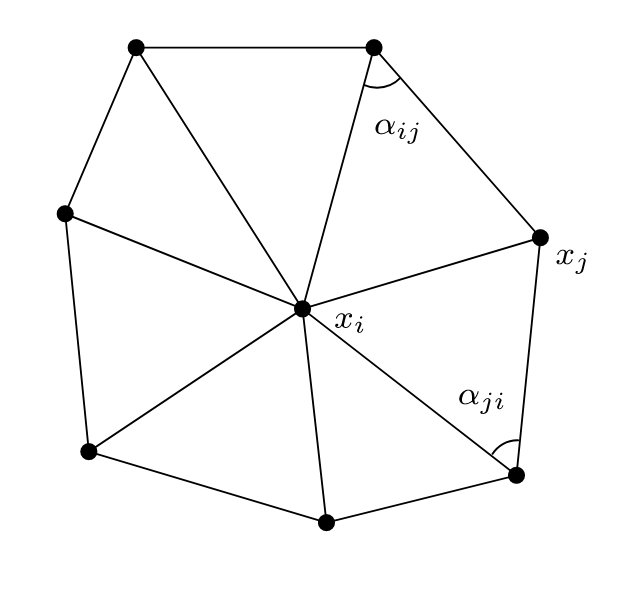
\includegraphics[width=0.4\linewidth]{resources/img/cotangent_approx.png}
	\caption{Berechnung der $\alpha$-Winkel für eine innere Kante~\cite{laplace_beltrami_paper}.}
	\label{fig:cotangent_approx}
\end{figure}

\begin{equation}
    \label{eq:cotangent_weight}
    v(x_i,x_j) = 
        \begin{cases}
            \cot{\alpha_{ij}}+\cot{\alpha_{ji}}\ & \text{for interior edges} \\
            \cot{\alpha_{ij}} & \text{for boundary edges}
        \end{cases}
\end{equation}

Aus den Kotangens-Gewichten aus Gleichung~\ref{eq:cotangent_weight} kann nun in Formel~\ref{eq:laplace_beltrami} der Laplace-Beltrami Operator in seiner Matrix-Form berechnet werden \cite{spd_solver_paper,laplace_beltrami_paper}. Dabei bescheibt $N(x_i)$ die Menge der benachbarten Vertices von $x_i$. Da für das Lösen der Gleichung~\ref{eq:bone_heat} lediglich die Matrix $(-\Delta+\textbf{H})$ benötigt wird, kann diese in der Implementierung direkt als eine Matrix erstellt werden. Die Normalisierungsfaktoren aus~\cite{spd_solver_paper} wurden hier weggelassen, da sie für diese Anwendung sowieso wegfallen.

\begin{equation}
    \label{eq:laplace_beltrami}
    \Delta_{ij}=
    \begin{cases}
        0 & i \neq j, x_j \notin N(x_i) \\
        v(x_i,x_j) & i \neq j, x_j \in N(x_i) \\
        -\sum_{x_j\in N(v_i)} v(x_i,x_j) & i = j\\
    \end{cases}
\end{equation}

Da die Matrix $\textbf{H}$ eine Diagonalmatrix ist und der Operator $\Delta$ eines Vertex durch seine direkten Nachbarn lokal definiert ist, ist die zu lösende Matrix extrem dünn besetzt. Durch die Euler-Charakteristik für Dreiecks-Netze ergeben sich nur ungefähr $7$ Einträge in der Matrix pro Reihe~\cite{spd_solver_paper}. Ein solches System lässt sich, wie in~\cite{spd_solver_paper} gezeigt, sehr effizient lösen, wenn es sich um eine SPD-Matrix (symetrisch positiv definit) handelt. Die Matrix ist durch die Konstruktion in Gleichung~\ref{eq:laplace_beltrami} symetrisch. Für die Lösung dieses Systems wurde in diesem Projekt die Bibliothek Eigen~\cite{eigen} verwendet, welche zahlreiche Methoden zur Matrix-Berechnung bereitstellt. Es wurde der Matrix-Solver \texttt{SparseLU} verwendet, welcher auf dünn besetzte SPD-Matrizen spezialisiert ist.

Durch die Lösung des Systems für jeden Bone $i$ erhalten wir einen Vektor $\textbf{w}^i$ aus Gleichung~\ref{eq:bone_heat}. Wir hängen jeden Vertex mit dem entsprechenden Gewicht an diesen Bone, falls das Gewicht größer als $0$ ist. Für die Verwendung der Gewichte in Unity mussten diese außerdem pro Vertex absteigend sortiert und normalisiert werden, sodass sie sich zu $1$ aufsummieren.